\chapter{جزئیات فنی پروژه}


\section{مقدمه}
\section{دورنمای کلی طرح}
همان‌طور که گفته شد، در این پروژه از ابزار های مختلفی استفاده شده است. برخی ابزارات دیگر نیز جهت ایجاد اتصال بین آن ابزار ها استفاده شده اند. در این بخش، این اجزا به تفصیل بررسی خواهد شد.
 
 هر کدام از این اجزا کار مشخصی را بر عهده دارند.
 شکل  
\ref{fig:block-diagram}
این ارتباط را نشان می‌دهد.

\begin{figure}[h!]
	\centering
	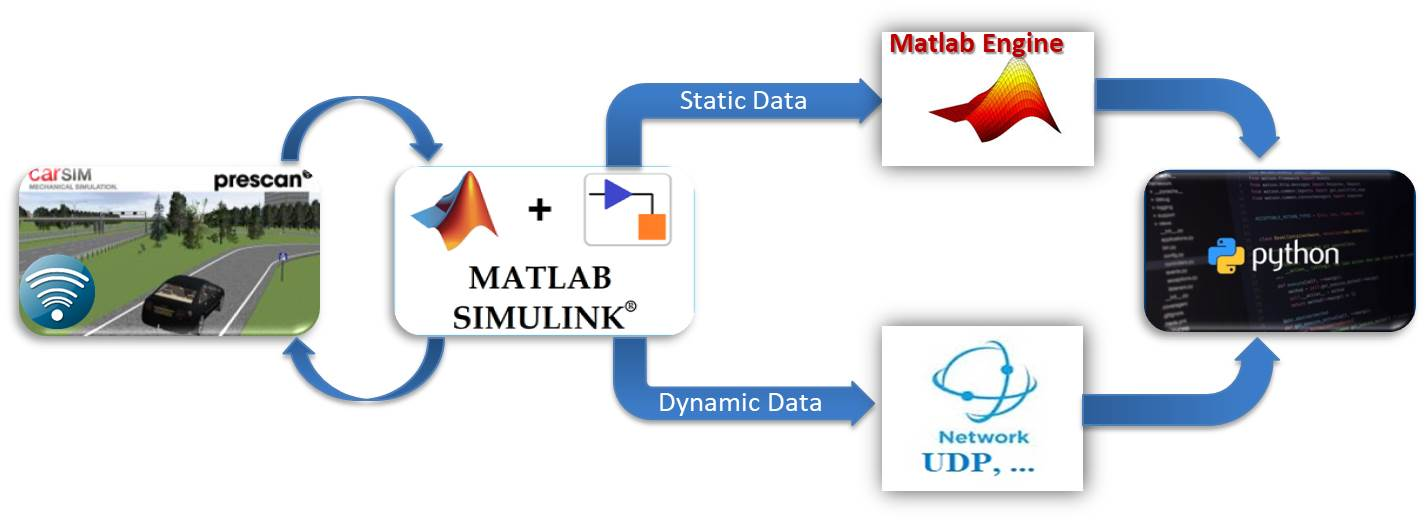
\includegraphics[width=1\linewidth]{Figures/block-diagram-white}
	\caption{بلوک دیالگرام لایه های کلی}
	\label{fig:block-diagram}
\end{figure}

در شکل 
\ref{fig:block-diagram}
از سمت چپ به راست اجزا یاد شده و نحوه ارتباط آن‌ها با‌یک‌دیگر را به‌خوبی نشان می‌دهد. این بلاک ها و ارتباط ها عبارتند از:

\begin{itemize}
	\item 
	اولین بلاک آن، نرم افزار \textbf{پری‌اسکن }می‌باشد. وظیفه اصلی این نرم افزار، شبیه سازی دینامیک یک اتومبیل و یا موتور و ... می‌باشد. همچنین ایجاد یک محیط گرافیکی زیبا و یک پنل کاربری گرافیکی برای ساخت ماشین ها از دیگر حسن های این نرم افزار است.
	
	فایل های مهم ایجاد شده توسط این بخش، \texttt{.pex} و \texttt{.pb} می‌باشد.
	
	\item
	بلاک بعدی ترکیبی از \textbf{متلب و سیمولینک }است. چرا که نرم افزار پری‌اسکن این امکان را دارد که برای کنترل و دسترسی بیشتر به قسمت های کنترلی مختلف، چیزی به نام \lr{API} ارائه می‌دهد. این \lr{API} یک فایل سیمولینک را در اختیار کابران قرار میدهد که در آن بلوک های مشخصی به یکدیگر متصل هستند و با مطالعه و تغییر آن بلوک ها می‌توان کنترل سیستم را به دست گرفت.
	
	فایل های مهم این بخش نیز در فرمت \texttt{.slx} و \texttt{.m} در دسترس هستند.
	
	همچنین \api یاد شده، دستورات دیگری را جهت دریافت داده های استاتیک محیط ساخته شده در این نرم افزار را به کاربران خویش در محیط متلب می‌دهد.

	\item
	دو بلوک بعدی، مربوط به اتصال بین متلب و یا سیمولینک با پایتون هستند. 
	
	بلوک بالایی این اتصال را بین داده های استاتیک شامل طول جاده و عرض هر لاین، موقعیت اولیه اتومبیل و جاده، و بسیاری اطلاعات دیگر که بسیاری از آن اطلاعات استفاده نشده اند زیرا در این پروژه مفید نبوده اند. این بلوک، فایل سیمولینک را تغییر نمی‌دهد.
	
	بلوک پایینی نیز با استفاده از روش های شبکه کردن، می‌تواند داده های پویا را از محیط سیمولینک به پایتون منتقل کند. این داده های پویا عبارتند از موقعیت و سرعت و اطلاعات دیگری از اتومبیل در حال حرکت، اطلاعات سنسورها و ... باشد.
	
	\item 
	بلوک بعدی پایتون است که خود شامل لایه های دیگری است که در شکل 
	\ref{fig:python-layers}
	به تفضیل بیان شده است. نکته جالب در آن این است که در آن لایه ها اثری نیز از دو بلوک پیشین آمده است. همچنین بخش اصلی کار، یا به عبارتی مغز و هوش این کار در این قسمت توسعه یافته است.
\end{itemize}
\subsection{تقسیم بندی وظایف هر بخش}
بخش اصلی کار که وظیفه آن تصمیم گیری و انتخاب مسیر درست توسط یک عامل
\LTRfootnote{Agent}
(که در این پروژه، عامل همان اتومبیل می‌باشد) در پایتون انجام می‌شود. وظیفه اصلی بخش متلب و سیمولینک و پری‌اسکن، ایجاد یک محیط شبیه سازی است. 

\begin{note}


این محیط شبیه سازی اهمیت زیادی در الگوریتم های یادگیری تقویتی دارد. زیرا در این الگوریتم ها یک «عامل» با «محیط
\LTRfootnote{Environment}
» در تعامل است. تعامل در این الگوریتم ها به معنای این است که «عامل» در یک «حالت
\LTRfootnote{State}
» قرار دارد. سپس متناسب با آن یک «حرکت
\LTRfootnote{Action}
» انجام می‌دهد. با این «حرکت»، «محیط» به آن یک مقدار «امتیاز» و یک «حالت» جدید بر‌می‌گرداند. 
بنابراین داشتن یک محیط شبیه سازی کامل و دقیق از اجزای ضروری کار است.

\end{note}

بخش های دیگر مربوط به ارتباط این قسمت ها به یک‌دیگر بودند که پیچیدگی های زیادی را رقم زده است.

به طور ساده‌تر و کلی‌تر می‌توان گفت که پایتون نقش «عامل» و پری‌اسکن نقش «محیط» را دارد.

\section{معرفی نرم افزار پری‌اسکن}
می‌توان در ابتدا گفت که این نرم‌افزار یک افزونه متلب و سیمولینک است اما توانایی زیادی که آن دارد باعث می‌شود که بگوییم این محصول از متلب و سیمولینک جعت رسیدن به هدف خود کمک می‌گیرد.

نرم افزار پری‌اسکن یکی از نرم افزار های بسیار قدرتمند در زمینه شبیه سازی مسایل مربوط به وسایل نقلیه است که می‌تواند حرکت یک ویله نقلیه را به طور خیلی دقیق و مناسب شبیه سازی کند. همچنین در کنار این وظیفه مهم، یک محیط گرافیکی مناسب را در اختیار کاربران خود قرار می‌دهد که از دیگر حسن های آن است.
شکل 
\ref*{fig:prescan-gallery} این توانایی ها را به تصویر کشیده است.
 
همچنین این نرم افزار یک سری فایل خروجی به کاربر می‌دهد که یکی از فایل های آن فایل سیمولینک است که اجازه تغییر و دسترسی به داخل برخی بلاک ها به ما کمک می‌کند که اطلاعات خود را از دل آن نرم افزار بیرون بکشیم.
\RTLfootnote{جهت کسب اطلاعات بیشتر و تهیه این نرم افزار به لینک زیر مراجعه کنید:
\\
\lr{\href{https://tass.plm.automation.siemens.com/prescan}{https://tass.plm.automation.siemens.com/prescan}}
}

از این رو در مقابسه با محیط های دیگر، محاسن زیادی را داشت که هدف این پروژه را در به کار‌گیری این ابزار تحت تاثیر قرار داد.



\begin{figure}
	\centering
	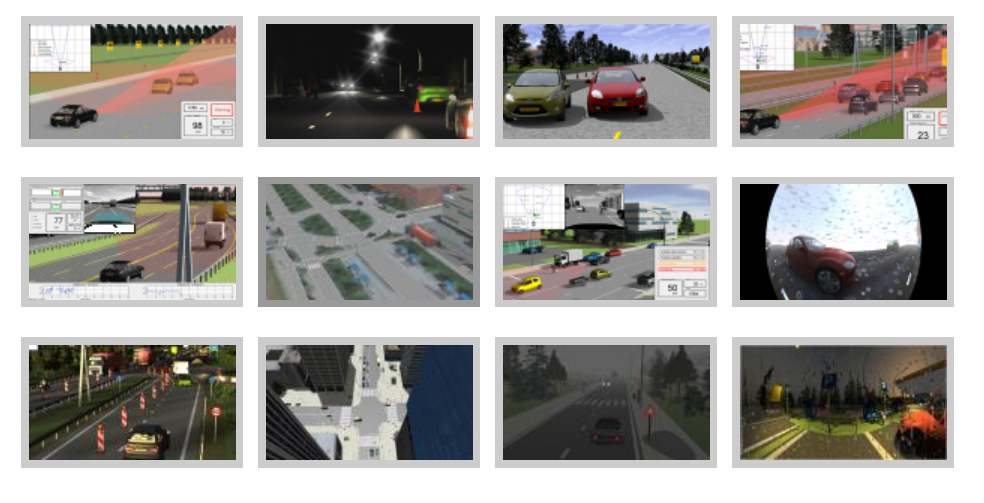
\includegraphics[width=0.8\linewidth]{Figures/Prescan-gallery}
	\caption{بخشی از توانایی های نرم افزار پری‌اسکن در شبیه سازی}
	\label{fig:prescan-gallery}
\end{figure}





\subsection{بخش های مختلف نرم افزار پری‌اسکن}
پس از دانلود و نصب نسخه \lr{8.5.0} این نرم‌افزار چهار آیکون مانند شکل 
\ref{fig:prescan-icons}
به محیط دسکتاپ اضافه می‌کند.  اصلی ترین آن ها 
\lr{PreScan Proccess Manager 8.5.0}
نام دارد.

\begin{figure}[h]
	\centering
	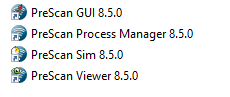
\includegraphics[width=0.4\linewidth]{Figures/prescan-icons}
	\caption{آیکون های اضافه شده بر روی محیط دسکتاپ پس از نصب پری‌اسکن}
	\label{fig:prescan-icons}
\end{figure}
 
 با انتخاب آن صفحه ای مانند زیر باز می‌شود.

\begin{figure}[h]
	\centering
	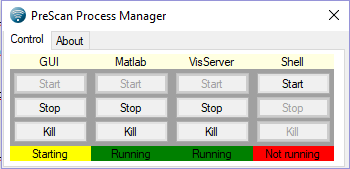
\includegraphics[width=0.5\linewidth]{Figures/Prescan-panel}
	\caption{پنل مدریت نرم‌افزار پری‌اسکن}
	\label{fig:prescan-panel}
\end{figure}

این پنجره شامل گزینه های زیر است:
\begin{multicols}{2}
\begin{itemize}
	\item \lr{GUI}
	\item \lr{VisServer}
	\item \lr{Matlab}
	\item \lr{Shell}
\end{itemize}
\end{multicols}

برای ایجاد یک محیط جدید باید \lr{GUI} را استارت کرد. پس از مدتی صفحه ای مانند شکل 
\ref{fig:prescan-gui}
باز می‌شود. 





\begin{figure}
	\centering
	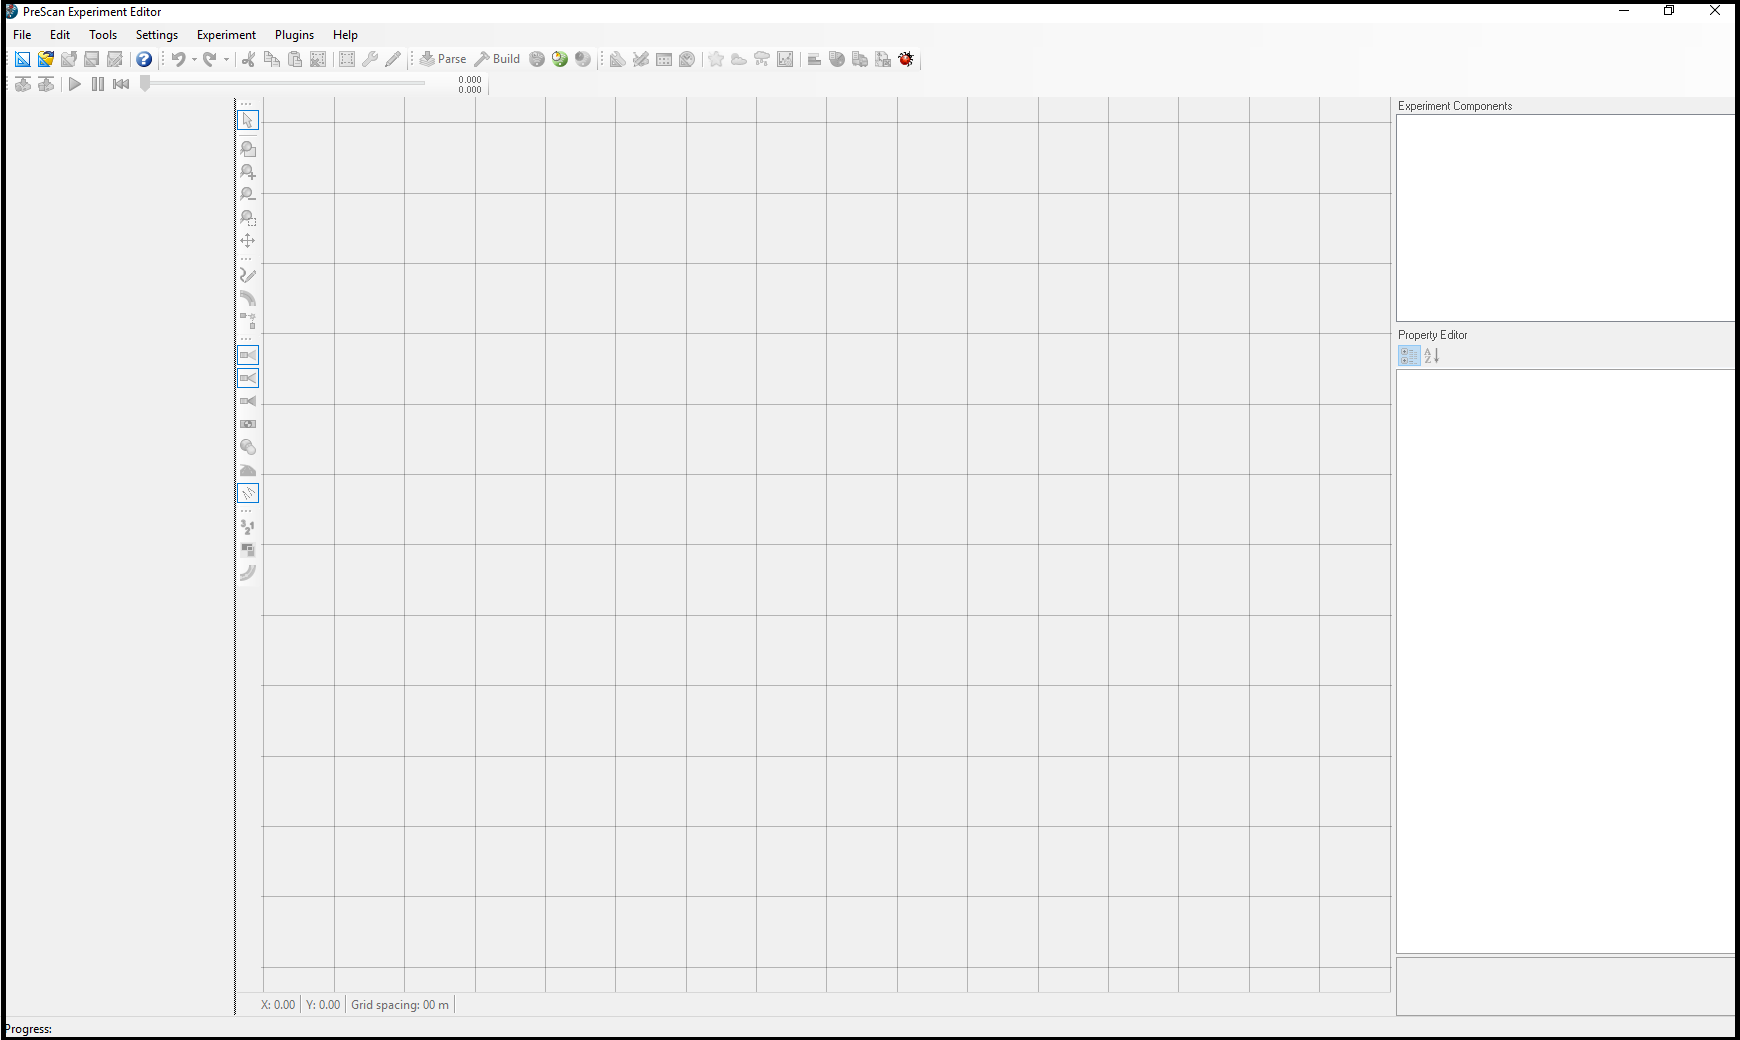
\includegraphics[width=0.7\linewidth]{Figures/Prescan-GUI}
	\caption{صفحه گرافیکی محیط پری‌اسکن}
	\label{fig:prescan-gui}
\end{figure}



پس از ایجاد مدل ها و ذخیره آن، فایل های \texttt{**.pex} و \texttt{**.pb} و \texttt{**\_cs.slx} ساخته می‌شود.
\RTLfootnote{علامت ** به معنای یک اسم مشترک در این سه فایل استفاده شده است. }

جهت استفاده از فایل سیمولینک باید در شکل 
\ref{fig:prescan-panel}
متلب را استارت کنید.
\begin{remark}
	برای اجرای فایل های سیمولینک خروجی، لازم است که متلب را فقط و فقط با استفاده از نرم افزار پری‌اسکن و با استفاده از پنل مدیریت نرم افزار معرفی شده در شکل 
	\ref{fig:prescan-panel}
	باز شود. در صورتی که به صورت مستقیم این کار انجام شود، به مشکل منتهی می‌شود.
\end{remark}


دو قسمت دیگر نیز در شکل 
\ref{fig:prescan-panel}
وجود دارد که نیازی به استارت کردن آن ها نیست و خودشان در صورت لزوم به صورت خودکار فراخوانی می‌شوند.


\subsection{فرمت های فایل های خروجی}
نرم‌افزار پری‌اسکن پس از ایجاد یک محیط جدید، فایل ها و پوشه های بسیار زیادی را ایجاد می‌کند. اما در خارج آن پوشه ها ۳ فایل وجود دارد که پسوند آن ها \texttt{**.pex} و \texttt{**.pb} و \texttt{**\_cs.slx} می‌باشد. علامت ** همان اسم پروژه‌ای است که ایجاد کرده ایم. هر یک از این فایل ها به یک بلوک از شکل 
\ref{fig:block-diagram}
مربوط می‌شود.

\begin{table}[h!]
\tableset{
%{\setcellgapes{0.5em}\makegapedcells
\begin{tabular}{|C{0.15\linewidth}|p{0.8\linewidth}|}
	\hline\rowcolor{lightgray}
	فرمت فایل
	&
	توضیحات 
	\\\hline\hline
	\texttt{**.pex} &	این فایل مربوط به اولین بلوک شکل
	\ref{fig:block-diagram}
	است و ارتباط مستقیم با \lr{GUI} دارد. برای تغییر محیط گرافیکی باید این فایل را باز کرد.
	\\ \hline   
	\texttt{**.pb} & این فایل برخی از اطلاعات فایل 
	\texttt{**.pex}
	را در اختیار دارد و با تغییر آن فایل این فایل نیز عوض می‌شود. این فایل حاوی اطلاعات استاتیک محیط ایجاد شده است و مهم ترین کاربرد آن در بلوک موتور متلب که در شکل 
	\ref{fig:block-diagram}
	نشان داده شده است می‌باشد. پایتون از طریق این فایل این اطلاعات را دریافت می‌کند.
	\\\hline
	\texttt{**\_cs.slx} &
	این فایل سیمولینک است که برای کار کردن با آن باید از پنل مدیریت شکل
	\ref{fig:prescan-panel}
	استفاده کرد. این فایل پس از ایجاد از فایل 
	\texttt{**.pex}
	مستقل می‌شود. این فایل خود قابلیت تغییر دارد و می‌توان بلوک‌های آن‌را در محیط سیمولینک تغییر داد و بلوک های دیگری به آن افزود.  در صورتی که فایل \texttt{**.pex} تغییر کند، این امکان را نیز دارد که از داخل خود سیمولینک با فشردن دکمه ای این تغییرات جدید اعمال شود بدون آن که به تغییرات خود کاربر لطمه ای وارد شود. در این پروژه این فایل، تغییرات بسیاری را تجربه کرد.
	\\\hline
\end{tabular}}
\caption{توضیحات فرمت فایل خروجی}
\label{tab:prescan-format}
\end{table}



جدول
\ref{tab:prescan-format}
توضیحات لازم را جهت آشنایی با این خروجی ها آورده است.

همچنین در بخش  
\ref{ch:fani|sec:simulink}
در مورد فایل \texttt{**\_cs.slx} توضیحات دقیق‌تری در مورد جزییات آن گفته خواهد شد.

\section{بررسی دقیق‌تر فایل سیمولینک}\label{ch:fani|sec:simulink}

فایل سیمولینک ایجاد شده توسط نرم افزار پری‌اسکن، قابلیت تغییر به دست کاربر را دارد. شکل 
\ref{fig:simulink-firstview}
فایل تغییر‌یافته مربوط به این پروژه را نشان می‌دهد.


\begin{figure}
	\centering
	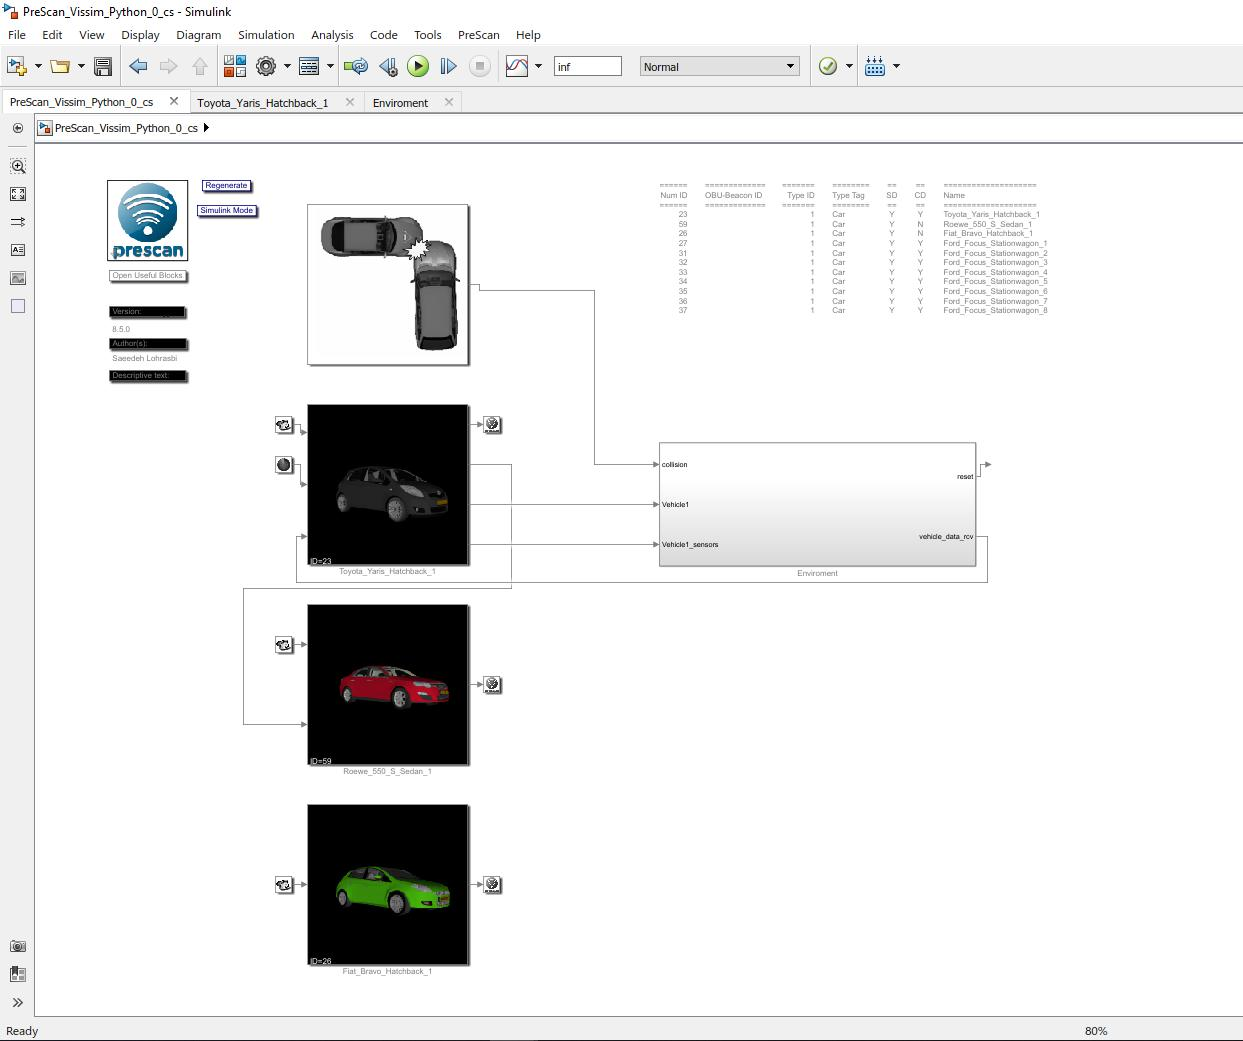
\includegraphics[width=0.7\linewidth]{Figures/simulink/first_view}
	\caption{فایل سیمولینک ایجاد شده توسط نرم افزار پری‌اسکن همراه با تغییرات}
	\label{fig:simulink-firstview}
\end{figure}




بلوک های سمت راست نشان داده شده در سمت راست شکل
\ref{fig:simulink-firstview}
توسط نرم افزار پری اسکن ایجاد شده است که البته دست‌خوش تغییراتی نیز بوده اند. 

در صورتی که با استفاده از محیط گرافیکی \lr{GUI} فایل \texttt{**.pex} تغییر کند، فایل سیمولینک تغییر نمی‌کند. در برخی موارد این تغییرات ممکن است منجر به پیغام خطا شود.

\begin{remark}\label{remark:Regenerate}
	در صورتی که فایل
	 \texttt{**.pex}
	 تغییر کند، برای اعمال این تغییرات، باید روی کلمه 
	 \lr{Regenerate}
	 که در شکل 
	 \ref{fig:simulink-generate}
	 آمده است، کلیک کرد. با این کار، تغییرات جدید اعمال می‌شود بی‌آن‌که تغییرات کاربر تحت تاثیر قرار بگیرد.
\end{remark}

\begin{figure}
	\centering
	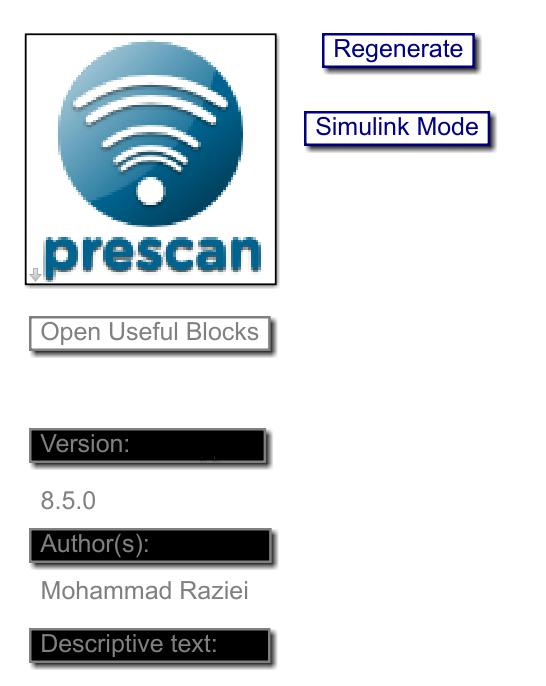
\includegraphics[width=0.4\linewidth]{Figures/simulink/generate}
	\caption{روش صحیح اعمال تغییرات روی فایل سیمولینک}
	\label{fig:simulink-generate}
\end{figure}

در شکل 
\ref{fig:simulink-generate}
همانطور که در نکته
\ref{remark:Regenerate} 
به آن اشاره شد، دکمه ای تحت عنوان 
\lr{Regenerate}
وجود دارد که استفاده از آن در همان نکته مشخص شده است. همچنین در این تصویر در زیر لوگوی برنامه پری‌اسکن، اطلاعاتی مانند شماره نسخه نرم افزار (که در این‌جا \lr{8.5.0} می‌باشد.)، نام نویسنده مشاهده می‌شود.

در شکل 
\ref{fig:simulink-firstview}
اولین بلوک سمت راست همان ماشینی است که ما آن‌را تحت کنترل گرفته‌ایم. اگه به آن وارد شویم، شکل 
\ref{fig:simulink-agent}
را مشاهده می‌کنیم.
در این تصویر ورودی و خروجی ها نقش خیلی مهمی دارند. این اطلاعات در جدول
\ref{tab:simuink-agent-io}
 آمده‌اند.



\begin{figure}[h!]
	\centering
	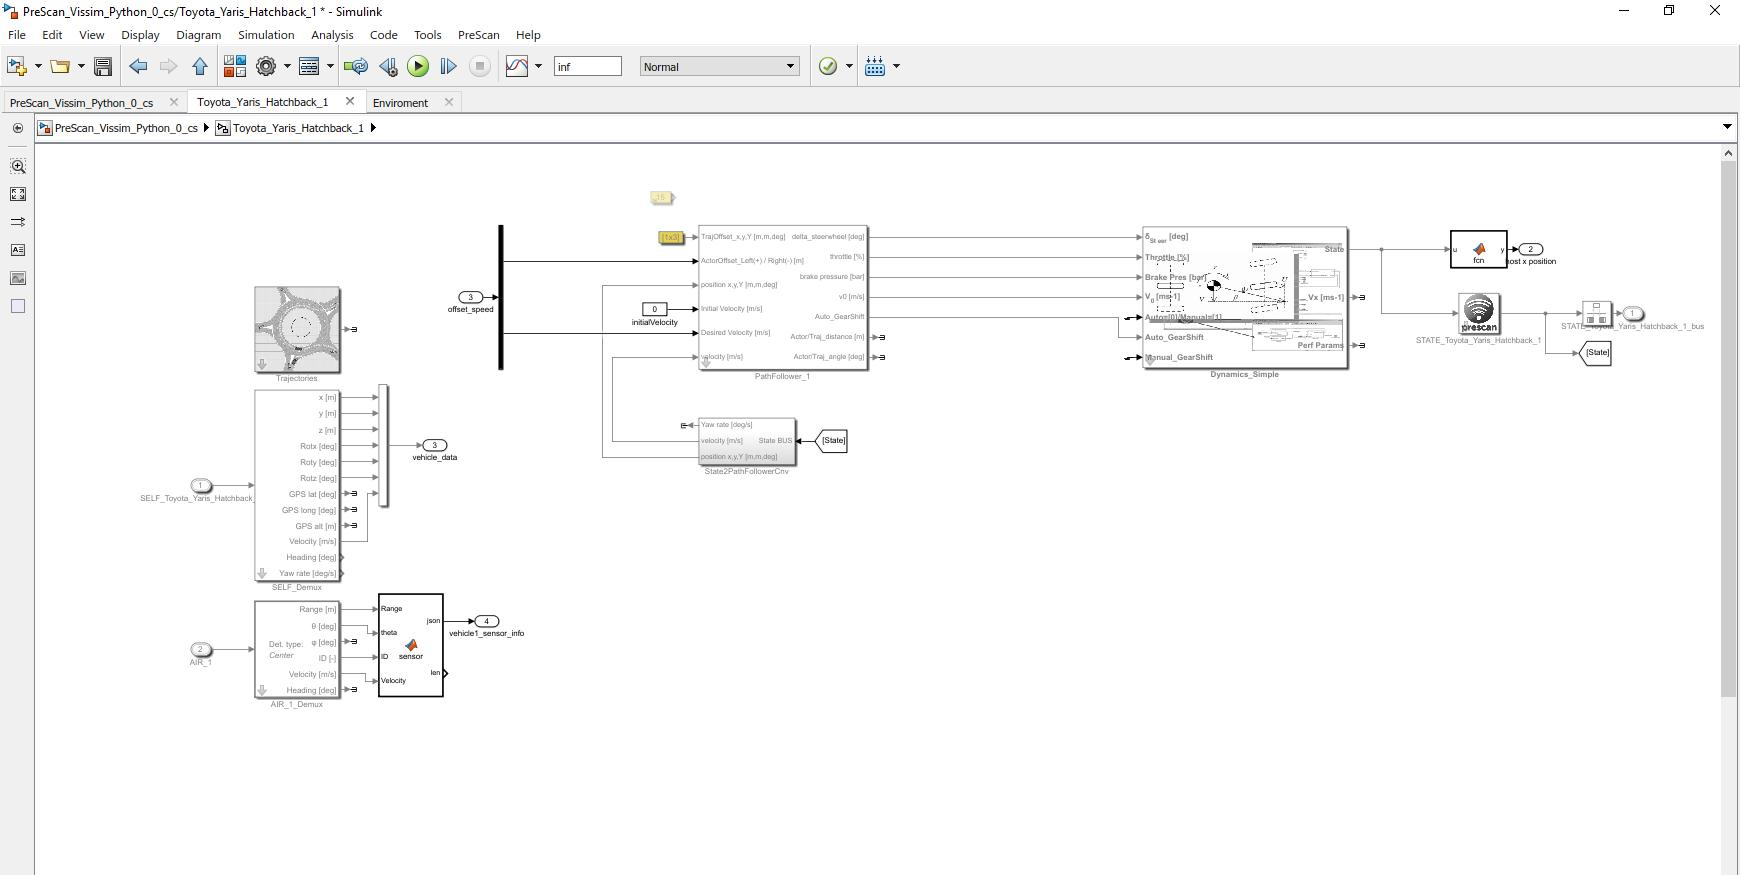
\includegraphics[width=1\linewidth]{Figures/simulink/agent}
	\caption{فایل سیمولینک - شبیه سازی اتومبیل}
	\label{fig:simulink-agent}
\end{figure}


\begin{table}[h!]
	\tableset{
		\begin{tabular}{|C{0.08\linewidth}|C{0.23\linewidth}|C{0.17\linewidth}|p{0.43\linewidth}|}
			\hline\rowcolor{lightgray}
			نوع & عنوان & بلوک مربوط & توضیحات
			\\\hline\hline
			خروجی &اطلاعات ماشین & \lr{SELF\_Demux} & اطلاعات ماشین، شامل اطلاعات موقعیت($x$،$y$ و$z$) و اطلاعات چرخش (حول $x$،$y$ و$z$) به همراه سرعت ماشین را خروجی می‌دهد. این 7 داده قبل از خروجی توسط یک \lr{mux} با یکدیگر ادغام می‌شوند.
			\\\hline
			خروجی& اطلاعات سنسور ماشین & \lr{AIR\_1\_Demux}  & اطلاعات سنسور \lr{V2C} را خروجی می‌دهد. از آنجا که این سنسور فاصله و زاویه و ...  تا ده ماشین نزدیک خود را می‌دهد. بنابراین هر‌یک از این اطلاعات یک بردار ده تایی است. برای فرستادن آن اطلاعات به خروجی، ابتدا آن‌ها را به  طریقی به فرمت جیسون
			\footnotemark%{json}
			تبدیل می‌کند و یک رشته کاراکتر با طول مشخص
			\footnotemark%{بعدا خواهید دید که مشخص بودن طول بسیار بسیار اهمیت دارد!}
			را خروجی می‌دهد.
			\\\hline
			ورودی & کنترل لاین و سرعت ماشین & \lr{PathFollower\_1} & دستورات کنترلی اتومبیل، شامل کدام خط بودن و مقدار سرعت نهایی، به صورت ورودی وارد یک \lr{demux} می‌شود و پس از جدا سازی، به بلوک مربوط متصل می‌شود.
			\\\hline
	\end{tabular}}
	\caption{بررسی ورودی ها و خروجی های مهم در شکل \ref{fig:simulink-agent}}
	\label{tab:simuink-agent-io}
\end{table}
\LTRfootnotetext[14]{json}
\RTLfootnotetext{بعدا خواهید دید که مشخص بودن طول بسیار بسیار اهمیت دارد!}


\subsection{معرفی بلوک 
\lr{Environment}
و بررسی جزییات آن
}

در جدول \ref{tab:simuink-agent-io} صرفا ورودی خروجی های مهم مورد بررسی قرار گرفته است. این ورودی ها و خروجی های مهم به یک بلوک دیگر منتقل می‌شود. بلوک 
\lr{Environment}
همان بلوک است که در شکل
\ref{fig:simulink-firstview}
نیز مشخص است و در شکل 
\ref{fig:simulink-env}
نیز از زاویه نزدیک تر با جزییات بیشتر می‌توان آن‌را مشاهده نمود.
%\code[matlab]{simulink-json-sensor.m}



\begin{figure}
	\centering
	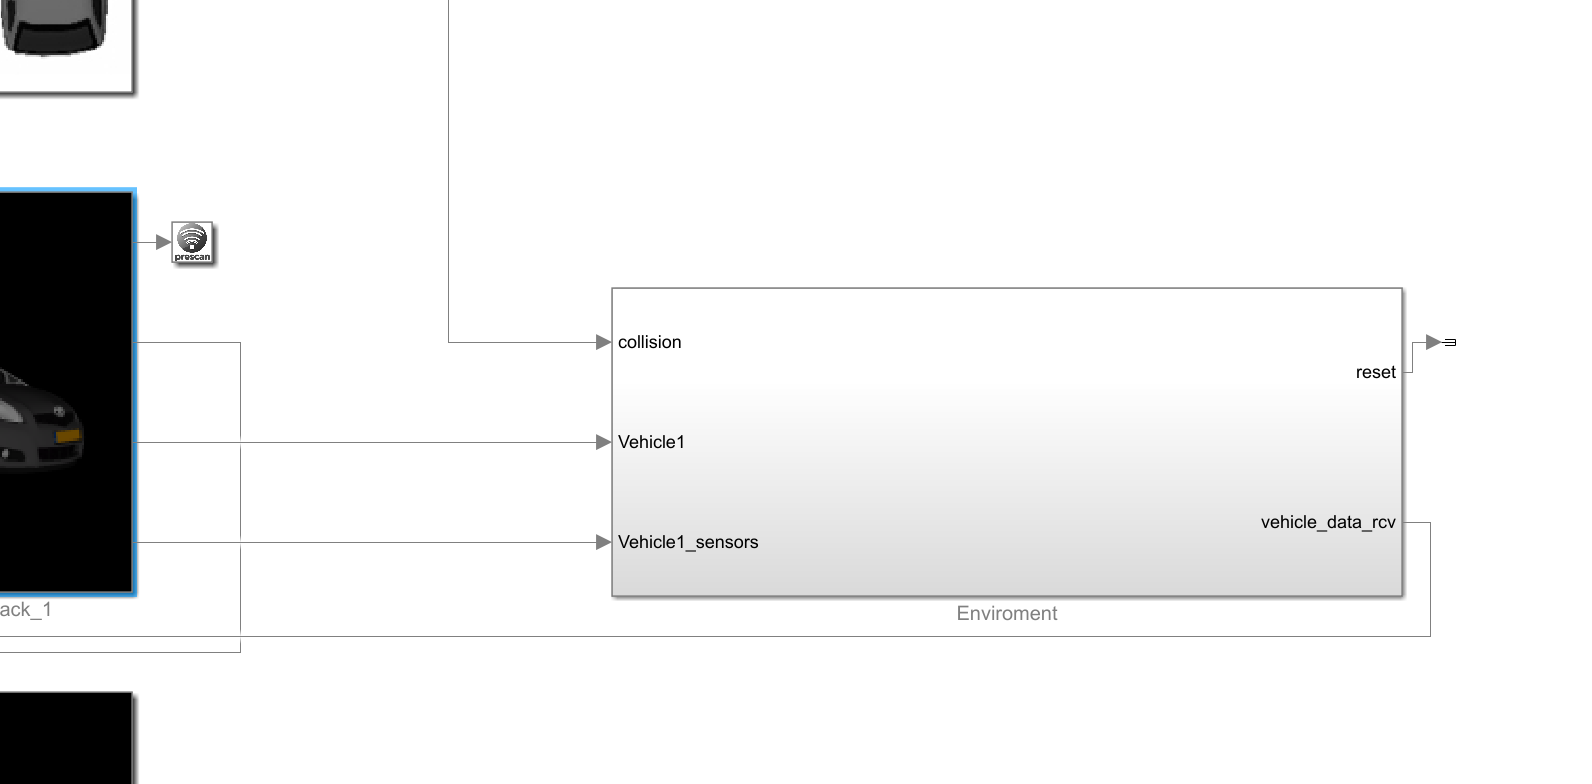
\includegraphics[width=0.7\linewidth]{Figures/simulink/simulink-Env}
	\caption{نگاهی از نزدیک به بلوک \lr{Environmnet}}
	\label{fig:simulink-env}
\end{figure}




وظیفه اصلی بلوک 
\lr{Environment}
جمع آوری اطلاعات محیط سیمولینک و همچنین ارسال دستورات کنترلی به آن هاست. اطلاعات جمع آوری شده از محیط سیمولینک شامل موارد زیر است.

\begin{itemize}
	\item 
	اطلاعات ماشینی که نقش «عامل» را در الگوریتم دارد.
	\item 
	اطلاعات سنسور های ماشین «عامل»
	\item 
	اطلاعات مربوط به تصادف کردن و کدوم ماشین با کدوم ماشین تصادف کرده است.	
\end{itemize}

این اطلاعات به صورت ورودی به این بلوک وارد می‌شود و دستورات کنترلی شامل کنترل لاین ماشین به همراه مقدار سرعت نهایی ماشینی که نقش «عامل» در الگوریتم دارد، از این بلوک خارج می‌شود.

پیشتر صحبت شد که وظیفه تصمیم گیری بر عهده کد پایتون است. با این حساب سیمولینک قدرت تشخیص و تصمیم گیری ندارد. از این رو وظیفه بلوک 
\lr{Environment}
نیز تصمیم گیری نمی‌باشد بلکه با تکنیک هایی سعی بر برقراری ارتباط با کد پایتون دارد. در حقیقت این بلوک نقش واسط بین سیمولینک و پایتون را دارد. این بلوک علاوه بر دستورات کنترلی لاین و سرعت، دستور «شروع کردن دوباره» و یا ریست را نیز دریافت می‌کند. با این دستور تمامی اطلاعات به حالت اول بر خواهد گشت و ماشین «عامل» به جای اول بر خواهد گشت و منتظر دستورات جدید می‌ماند.

شکل 
\ref{fig:block-diagram}
توضیح بسیار کلی  در مورد این نحوه ارتباط نشان داده است و در شکل 
\ref{fig:inside-environment}
جزییات بیشتری را در مورد داخل این بلوک را نشان می‌دهد.


\begin{figure}
	\centering
	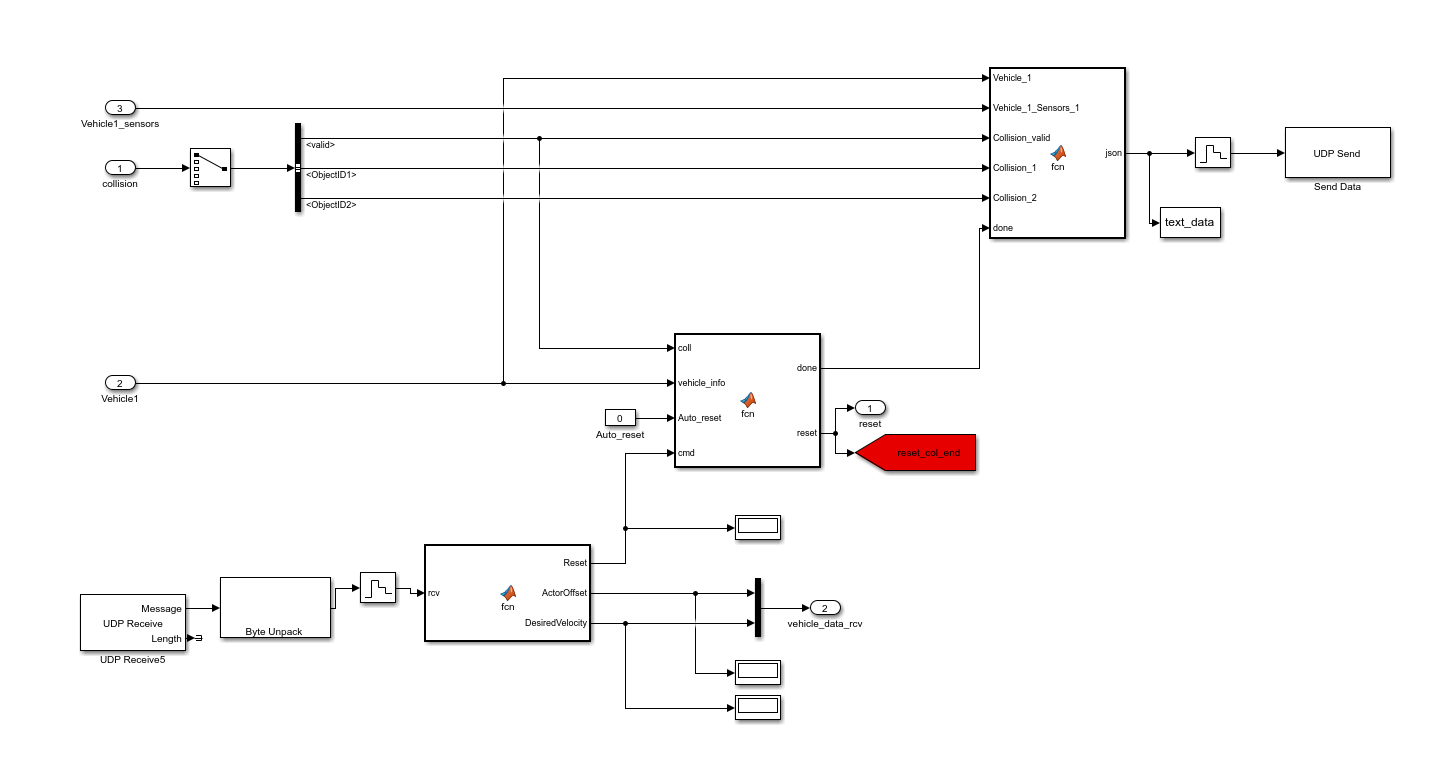
\includegraphics[width=0.95\linewidth]{Figures/simulink/inside-Environment}
	\caption{فایل سیمولینک - داخل بلوک \lr{Environment}}
	\label{fig:inside-environment}
\end{figure}

اگر به شکل 
\ref{fig:inside-environment}
دقت شود دو بلوک 
\lr{UDP}
دیده می‌شود. (بلوک 
\lr{UDP Send}
در بالا سمت راست و بلوک 
\lr{UDP Receive}
در پایین سمت چپ شکل 
\ref{fig:inside-environment}
)
این دو بلوک برای فرستادن داده های مورد نیاز به پایتون و گرفتن دستور های کنترلی از پایتون در سیمولینک تعبیه شده اند.

\begin{note}
	
اگر نمودار شکل
\ref{fig:block-diagram}
در نظر داشته باشیم، خواهیم یافت که این بلوک در شاخه پایینی ارتباط بین سیمولینک و پایتون قرارا دارد که از روش های شبکه کردن بین این دو انجام می‌شود. این بلوک صرفا داده‌های پویا را از متلب به سیمولینک انتقال می‌دهد و با داده‌های استاتیک کاری ندارد. 

\end{note}

 در جدول
\ref{tab:Reciver-Send}
 اطلاعات دقیق شبکه برای این دو بلوک دیده می‌شود. گفتنی است که این داده ها به نحوه مناسب کد شده‌اند تا تنها با استفاده از این دو بلوک بتوان داده ها را منتقل کرد.


\begin{table}
\tableset{
	\begin{tabular}{|c|c|c|c|c|}
		\hline\rowcolor{lightgray}
		نام بلوک & نوع بلوک & \lr{IP} & \lr{Port} & توضیحات
		\\\hline\hline
		\lr{UDP Receiver} & گیرنده & \lr{localhost} & 8070 &
		\\\hline
		\lr{Send Data} & فرستنده & \lr{localhost} & 8031 &
		\\\hline
	\end{tabular}}
	\caption{اطلاعات بلوک های فرستندگی گیرندگی در سیمولینک}
	\label{tab:Reciver-Send}
\end{table}


روش کد شدن
\LTRfootnote{Encoding}
قبل از ارسال و یا دریافت در این دو بلوک کاملا با یکدیگر متفاوت هستند. این کار توسط بلوک‌های قبل و بعد دو بلوک مذکور انجام می‌شود. 



در شکل 
\ref{fig:inside-environment}
سه بلوک تابع متلب 
\LTRfootnote{Matlab-function block}
   وجود دارد که از مهم‌ترین نقش را دارند. این نقش‌ها در ادامه توضیح توضیح مفصل داده شده‌اند.
   
   خلاصه این وظایف در زیر آمده است:
   
   \begin{itemize}
   		\item \textbf{بلوک فرستنده} :
   		این بلوک در سمت بالا سمت راست تمام اطلاعاتی که به بلوک کلی 
   		\lr{Environment}
   		وارد می‌شود را به نحوی مناسب به همراه متغیر \texttt{done} که از یک تابع متلب دیگر خارج می‌شود را برای پایتون طی ساختار مشخصی (جیسون) ارسال می‌کند. موضوع به صورت بسیط در بخش
   		\ref{ch:fani|sec:simulink|sub:json}
   		مورد بررسی قرار گرفته است.
   		\item \textbf{بلوک گیرنده} :
   		این بلوک تنها وظیفه آن این است که داده هایی که پس از بلوک \lr{Byte Unpacking} آمده است ، را انتخاب می‌کند که هر یک از این دیتا ها چه مفهومی هستند. از آن‌جا که ۳ داده کنترلی (لاین و سرعت و ریست) از طرف پایتون ارسال می‌شود، بلوک \lr{Byte Unpacking} وظیفه این ۳ داده را به فرمت \texttt{double} در می‌آورد (این فرمت در سمت پایتون نیز به همین شکل قرار داد شده‌است). بنابراین این بلوک \lr{Byte Unpacking} است که کار اصلی را انجام می‌دهد و تنها وظیفه این بلوک تفکیک و اسم گذاری بر‌روی خروجی بلوک \lr{Byte Unpacking} است.
   
   		\item \textbf{بلوک محاسبه تمام شدن و ریست کردن} :
   		این بلوک با دو خروجی مهم می‌دهد. یکی از آن خروجی ها \texttt{done} است که توسط بلوک فرستنده نیز برای پایتون ارسال می‌شود. و مقدار دیگری را که خروجی می‌دهد دستور ریست کردن است. این دستور در لبه مثبت (از صفر به یک برسد) ریست می‌کند. منطق این بلوک یک منطق باینری است که در شکل 
   		\ref{fig:done-reset-logical}
   		روش محاسبه آن نیز آمده است. 
   		همچنین این بلوک یک مقدار به اسم \texttt{Auto\_reset\_flag} نیز به عنوان ورودی دریافت می‌کند. این مقدار که می‌تواند صفر و یا یک باشد، تصمیم می‌گیرد که در صورتی که \LRE{\texttt{done = 1}} شد آیا ریست کند و یا ریست نکند. اگر یک باشد ریست می‌کند وگرنه منتظر رسیدن دستور از پایتون می‌ماند.
   		
   \end{itemize}

\begin{figure}
	\centering
	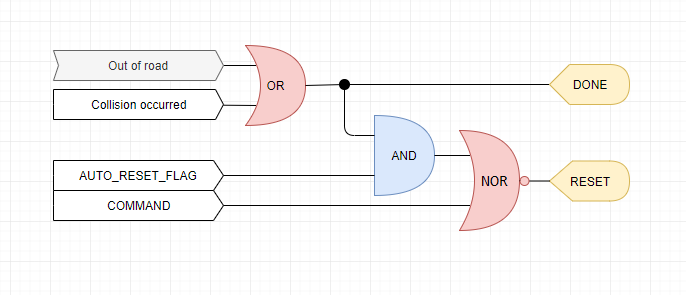
\includegraphics[width=0.7\linewidth]{Figures/done-reset-logical}
	\caption{منطق محاسبه تمام شدن و دستور ریست کردن}
	\label{fig:done-reset-logical}
\end{figure}

   
\subsection{بررسی ساختار داده های ارسالی  و کد آن در سیمولینک}\label{ch:fani|sec:simulink|sub:json}
   
   بلوک فرستنده در شکل
   \ref{fig:inside-environment}
   اطلاعات دریافت شده را طی ساختار مشخصی به ساختار جیسون در می‌آورد.
   نمونه ای از این ساختار در شکل
   \ref{fig:block-diagram}
    آمده است.
%\begin{figure}
%	\centering
%	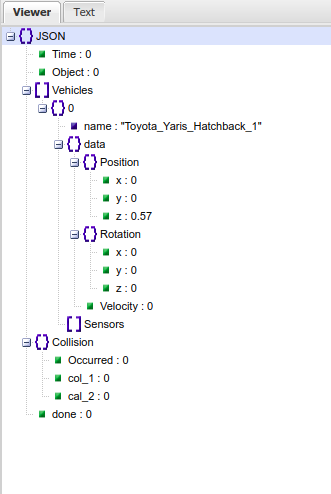
\includegraphics[height=8cm]{Figures/simulink/json-env}
%	\caption{}
%	\label{fig:json-env}
%	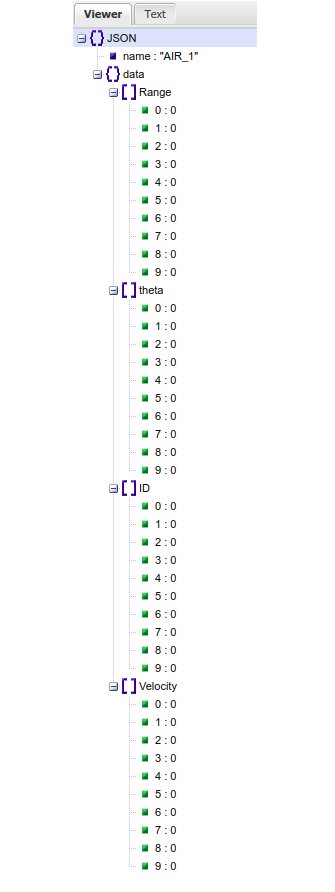
\includegraphics[height=8cm]{Figures/simulink/json-sensor}
%	\caption{}
%	\label{fig:json-sensor}
%	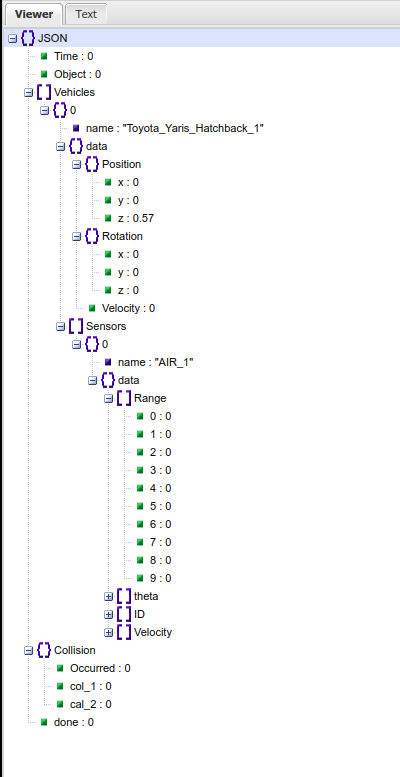
\includegraphics[height=8cm]{Figures/simulink/json-total}
%	\caption{}
%	\label{fig:json-total}
%\end{figure}
   
   
   
%\begin{latin}
%\begin{lstlisting}[language=json]
%'{"Time":0,"Object":0,"Vehicles":[{"name":"Toyota_Yaris_Hatchback_1","data":{"Position":{"x":0.00000e+00,"y":0.00000e+00,"z":5.70000e-01},"Rotation":{"x":0.00000e+00,"y":0.00000e+00,"z":0.00000e+00},"Velocity":0.00000e+00},"Sensors":[{"name":"AIR_1","data":{"Range":[0.00000e+00,0.00000e+00,0.00000e+00,0.00000e+00,0.00000e+00,0.00000e+00,0.00000e+00,0.00000e+00,0.00000e+00,0.00000e+00],"theta":[0.00000e+00,0.00000e+00,0.00000e+00,0.00000e+00,0.00000e+00,0.00000e+00,0.00000e+00,0.00000e+00,0.00000e+00,0.00000e+00],"ID":[0.00000e+00,0.00000e+00,0.00000e+00,0.00000e+00,0.00000e+00,0.00000e+00,0.00000e+00,0.00000e+00,0.00000e+00,0.00000e+00],"Velocity":[0.00000e+00,0.00000e+00,0.00000e+00,0.00000e+00,0.00000e+00,0.00000e+00,0.00000e+00,0.00000e+00,0.00000e+00,0.00000e+00]}}]}],"Collision":{"Occurred":0,"col_1": 0,"cal_2": 0},"done":0}'
%\end{lstlisting}
%\end{latin}
   
  
   
   
   

\begin{figure}[h!]
  	\centering
  	\subfigure[اطلاعات خام جیسون کلی]{%
  		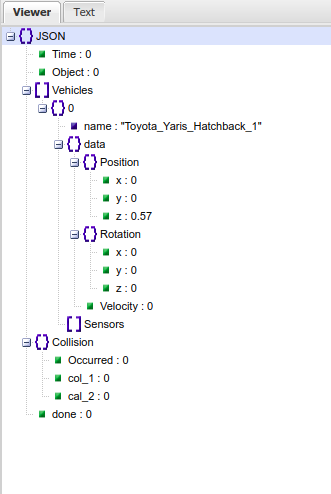
\includegraphics[height=8cm]{Figures/simulink/json-env}
   		\label{subfig:json-env}
  	}
%  	\hspace*{1.5cm} % space between two figures
  	\subfigure[جیسون سنسور]{%
  		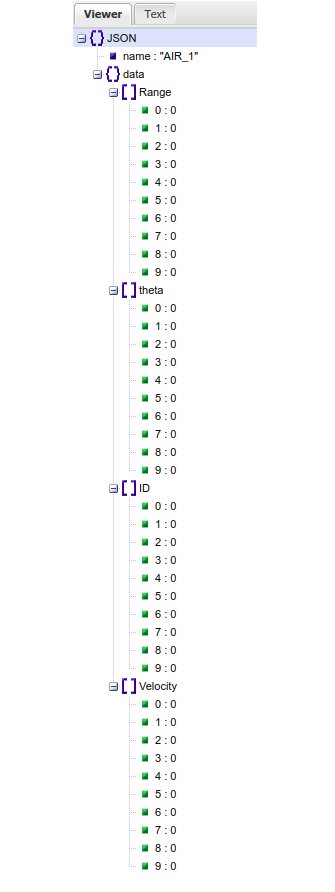
\includegraphics[height=8cm]{Figures/simulink/json-sensor}
   		\label{subfig:json-sensor}
  	}
%  	\\ % place in new line
%  	\hspace*{1.5cm} % space between two figures
  	\subfigure[شکل ادغام شده ]{%
  		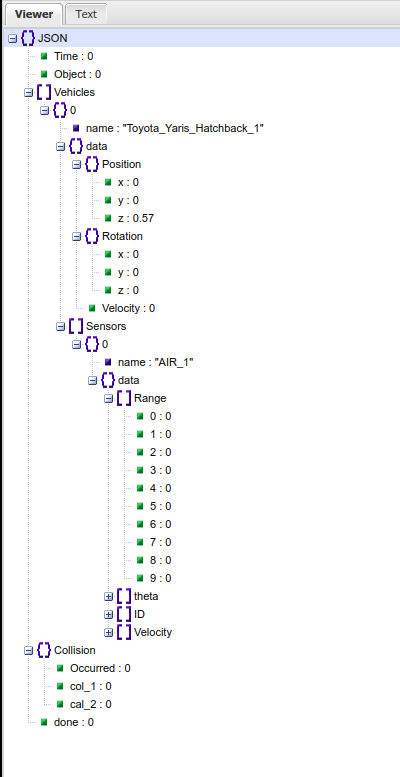
\includegraphics[height=8cm]{Figures/simulink/json-total}
   		\label{subfig:json-total}
  	}
  	\caption[ساختار جیسون برای بلوک های سیمولینک]{%
  		تصویر
  	\subref{subfig:json-env}
  	نحوه ساختار‌دهی کلی در بلوک تابع متلب واقع در زیرسیستم 
	\lr{Environment}
	را نشان می‌دهد. در این قسمت اطلاعات ماشین شامل دو قسمت \lr{data} و \lr{Sensors} است. اطلاعات سنسور های این ماشین  از تصویر \subref{subfig:json-sensor} تامین می‌شود. این ساختار در همان زیرسیستم ماشین تبدیل به جیسون شده و برای زیر‌سیستم \lr{Environmnet} ارسال می‌شود. قسمت سنسور یک آرایه است تا بتوان چندین سنسور مختلف را برای آن ارسال کرد. بنابراین ساختاری مانند تصویر \subref{subfig:json-total} باید را در نهایت برای پایتون ارسال می‌کند.
	\footnotemark
  	}
  	\label{fig:json-total}
\end{figure}
	\RTLfootnotetext{این عکس با استفاده از سایت
		\lr{\href{http://jsonviewer.stack.hu/}{http://jsonviewer.stack.hu/}}
	تهیه شده است.}
شکل \ref{subfig:json-sensor} همان ساختاری است که پیشتر در مورد آن صحبت شد. با توجه به این که این ساختار (در ادامه خواهید دید که) در اطلاعات سنسور ماشین به کار گرفته می‌شود و هر سنسور ممکن است اطلاعات خاص خود را داشته باشد. برای یکسان‌سازی این اطلاعات، در اولین لایه دو گزینه \lr{data} و \lr{name} را به طور قرار دادی بین همه سنسور ها یکسان است تا در کد پایتون بتوان با توجه به اسم آن ها ادامه ساختار که در \lr{data} می‌باشد، قابل تشخیص باشد. اما از آن‌جا که صرفا از اطلاعات یک سنسور استفاده شده است این شکل ساختار‌دهی تنها یک گزینه برای توسعه های آتی آن است.

در این ساختار ۴ اطلاعات نشان داده شده که هر یک از آن اطلاعات خود یک بردار ۱۰ تایی است، برای پایتون ارسال می‌شود. 

شکل 
\ref{subfig:json-env}
ساختار کلی است که محیط \lr{Environmnet} از آن استفاده می‌کند. در این بلوک علاوه بر داده هایی مانند اطلاعات ماشین و سنسورش، اطلاعات تصادف و اطلاعات تمام شدن و یا نشدن شبیه سازی که پیش‌‌تر در مورد آن اطلاعات صحبت شد، دو اطلاعات اضافه دیگر نیز می‌فرستد.
\begin{itemize}
	\item \texttt{Time} :
	زمان شبیه سازی را همراه با دیتا دیگر ارسال می‌کند و به اصلاح یک ساختار زمانی ایجاد می‌شود.
	\LTRfootnote{Time-struct}
	\item \texttt{Object} :
	این عبارت کمک به کد پایتون می‌کند که ماشین هدف و یا عامل را از بین ماشین های موجود در لیست \texttt{Vehicles} بیابد. 
	\RTLfootnote{از آنجایی که در این پروژه  لیست \lr{Vehicles} یک آبجکت بیشتر ندارد، پس این بخش نیز صرفا ظرفیت توسعه‌پذیری این کد را بالا می‌برد.}
\end{itemize}

در نهایت با ادغام شدن اطلاعات سنسور نیز، ساختار کلی به شکل \ref{subfig:json-total} در خواهد آمد . در بخش
\ref{ch:fani|sec:chalenges}
از برخی از چالش های ساختاردهی کردن به این شکل، صحبت خواهد شد. همچنین خروجی نهایی آن نیز را می‌توانید در 
\hyperref[code:json]{همان بخش}
 بیابید.

\section{بررسی جزییات بخش پایتون}\label{ch:fani|sec:python}
بارها اشاره شد که پایتون بخش اصل تصمیم‌گیری را برعهده دارد. در بخش 
\ref{ch:fani|sec:simulink}
سعی شد تا به نحو مناسبی دیتای محیط شبیه‌سازی را به پایتون منتقل کند و دستورات کنترلی را نیز از پایتون به محیط شبیه‌سازی ارسال کند. در این بخش بر روی مفاهیم پایتونی آن مانور می‌دهیم.

از آن‌جا که کد پایتون باید به سیمولینک متصل شود و دیتا را به الگوریتم کنترلی خود (که از الگوریتم های یادگیری تقویتی استفاده شده است) ، برساند و از آن جا دستورات را دریافت کتد و به سیمولینک برساند، نیازمند لایه هایی است که هر لایه بخشی از این کار ها انجام دهد.

\subsection{معرفی لایه های کد پایتون}\label{ch:fani|sec:python|sub:layers}
کد پایتون از لایه های مختلف تشکیل شده است. از هر لایه به لایه بعدی سطح زبان بالاتر می‌رود. این لایه ها در شکل 
\ref{ch:fani|sec:python|sub:layers}
مشخص شده اند. در لایه های ابتدایی، سطح استفاده از دستورات بسیار ابتدایی است و در هر لایه با تعریف توابع و کلاس هایی این امکان را ایجاد کرده اند که بدون در نظر گرفتن این که در سطوح پایین‌تر چه اتفاقاتی می‌افتد، در سطوح بالاتر از آن امکانات استفاده کرد. در ادامه این بحث مفصل توضیح داده خواهد شد.



\begin{figure}
	\centering
	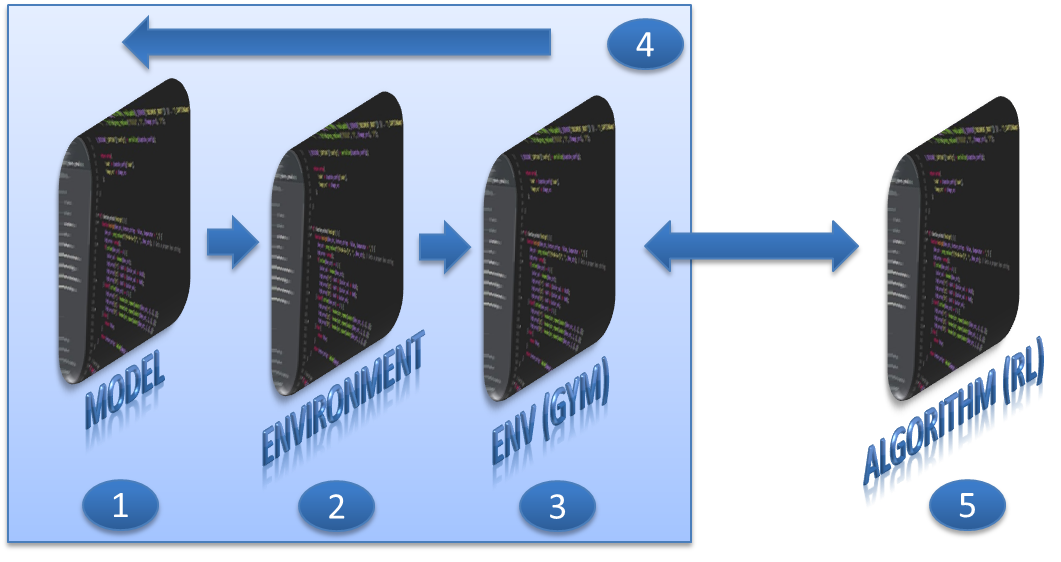
\includegraphics[width=0.8\linewidth]{Figures/python-layers-white}
	\caption{بلوک دیالگرام لایه های پایتون}
	\label{fig:python-layers}
\end{figure}
در شکل 
\ref{fig:python-layers}
۴ لایه برنامه نویسی شده با ۵ عدد نشان داده شده است. توضیحات زیر متناسب با هر‌یک از این شماره ها در نظر گرفته شده اند:




\begin{circlelist}
	\item \textbf{\lr{Model}} :
	در این لایه، با استفاده از موتور متلب با متلب و سیمولینک ارتباط برقرار می‌کند و با این ارتباط دو وظیفه بسیار مهم را انجام می‌دهد. 
	\begin{alphabetlist}
		\item 
		ساخت مدل هایی مانند اتومبیل و جاده و دریافت اطلاعات ضروری آن ها در متلب
		\item 
		تعریف کلاس \lr{sim} و ارسال دستوراتی مانند شروع کردن، توقف کردن، مکث کردن، ادامه دادن و ... به سیمولینک.
	\end{alphabetlist}
این لایه صرفا از اطلاعات استاتیک سیمولینک استفاده می‌کند.

	\item \textbf{\lr{Environment}} :
	این لایه برای ارتباط با زیرسیستم \lr{Environment} که پیشتر آن‌را در شکل 
	\ref{fig:simulink-env}
	مشاهده کردید، ساخته شده است. در این لایه با استفاده از ابزار هایی که لایه 
	\lr{Model}
	در اختیار آن قرار می‌دهد، به سادگی آبجکت هایی ماند ماشین و جاده را می‌سازد و با استفاده از اطلاعات شبکه که در جدول 
	\ref{tab:Reciver-Send}
	آمده است، با سیمولینک ارتباط برقرار می‌کند و آن اطلاعات پویا را دریافت می‌کند و دستورات کنترلی را برای آن ارسال می‌کند.
	
	این لایه از موتور متلب استفاده نمی‌کند بلکه از روش های شبکه ای استفاده می‌کند. 
	\item \textbf{\lr{Env}} :
	این لایه یک آبجکت از کلاس 
	\lr{Environment}
	را دریافت می‌کند و تمامی نیاز های خود را در مورد هر مسیله‌ای که به ارتباط با محیط متلب و یا سیمولینک به آن واگذار می‌کند و تمرکز آن برروی مفاهیم یادگیری تقویتی مانند 
	 \begin{enuminline}
	 	\item فضای مشاهده
	 	\LTRfootnote{Observation space}
	 	\item فضای حرکت
	 	\LTRfootnote{Action space}
	 	\item  تعریف حرکت
		\item تعریف حالت 
		\item تعریف امتیاز
 	\end{enuminline} 
 و ... می‌باشد.
 
	
	\item \textbf{\lr{gym}} :
	در نهایت یک مجموعه داریم که هر یک وظایف مربوط به خود را دارند. در این قسمت کد ما که در لایه \lr{Env} به \lr{gym} نزدیک شده است، با فراخوانی لایه های پیشین به ترتیب از بالا به پایین (از نظر سطح) فراخوانی می‌شود و در هر لایه آبجکت‌هایی از کلاس‌های موجود در لایه پایین تر فراخوانی می‌شود. از این رو جهت پیکان بر عکس است. 
	
	در مورد \lr{gym} در فصل 
	\ref{ch:openai-gym}
	به صورت مفصل بحث شده‌است.
	
	\item \textbf{\lr{Algorithm}} :
	در لایه های پیشین سینتکس کد \lr{gym} ایجاد شده است و این لایه بر توسعه الگوریتم های یادگیری تقویتی که در فصل 
	\ref{ch:RL}
	مورد بررسی مفصل قرار گرفته است، تمرکز دارد.
	
	می‌توان گفت این لایه نقش رییس و یا مغز کار را دارد و باقی لایه ها کارگرانی هستند که وظیفه دارند که اطلاعات را به شکلی مناسب این لایه، برای آن منتقل کنند.
\end{circlelist}	


\section{بررسی دقیق تر برخی چالش های فنی پروژه}\label{ch:fani|sec:chalenges}



\code[json,label={code:json}]{structure-string.json}

   








%\thispagestyle{empty}
%
%\section{مقدمه}
%
%فصل مقدمه یک پایان نامه، با بیان نیاز موضوع، تعريف مسئله و اهمیت آن در یک یا چند بند (پاراگراف) آغاز مي‌شود\footnote{شروع مقدمه نبايد چنان طولاني باشد كه هدف اصلي را تحت‌ تاثير قرار دهد.}  و با مرور پيشينه موضوع (سابقه کارهای انجام‌شده پیشین که ارتباط مستقیمی با مسئله مورد بررسی دارند) ادامه مي‌يابد. سپس در یک یا دو بند توضیح داده مي‌شود كه در این پایان نامه، چه ديدگاه يا راهكار جدیدي نسبت به مسئله (موضوع) مورد بررسي وجود دارد. به‌عبارت دیگر نوآوری‌ها به‌صورت کاملاً شفاف و صریح بیان می‌شود. در ادامه ممکن است به نتايج بدست‌آمده نیز به‌طور مختصر و کلی اشاره ‌شود. در آخرین بند از مقدمه به محتواي فصل‌هاي بعدي پایان نامه به‌اختصار اشاره مي‌شود.\\
%برای مشاهده دستورالعمل کامل دانشگاه صنعتی امیرکبیر(پلی تکنیک تهران) به \cite{zakeri} یا به سایت
%%
%\href{http://library.aut.ac.ir/Thesis%20Guide}{کتابخانه دانشگاه صنعتی امیرکبیر(پلی تکنیک تهران)}%
%مراجعه نمایید.
%
%نگارش صحيح يک پایان نامه در فهم آسان آن بسيار موثر است. در اين فصل مهمترین قواعد نگارشی که باید مورد توجه جدی نگارنده قرار گیرد، به اختصار بیان می‌شود. اين قواعد را مي‌توان در محورهای اصلی زير دسته‌بندی کرد:
%\begin{itemize}
%\item
%فارسی نویسی
%\item
%رعایت املای صحيح 
%\item
%رعایت قواعد نشانه‌گذاری
%\end{itemize}
%\section{فارسی نویسی}
%در حد امکان سعی کنيد به جاي کلمات غير‌فارسی از معادل فارسی آنها استفاده کنيد، به‌ويژه در مواردی که معادل فارسی مصطلح و رايج است‌.‌ به‌طور مثال استفاده از کلمه «لذا» به‌جای «برای همين» يا «به‌همين دليل» توجيهی ندارد‌. همچنين کلمه «پردازش» زيباتر از «پروسس» و معادل فارسی «ريز‌پردازنده» مناسب‌تر از «ميکروپروسسور» است‌.‌ در اين‌گونه موارد چنانچه احتمال عدم آشنايی خواننده با معادل فارسی وجود دارد، يا اصطلاح غير‌فارسی معمول‌تر است، در اولين ظهور کلمه فارسی، اصل غير‌فارسی آن به‌صورت پاورقي آورده شود‌.‌ اگر به‌ناچار بايد کلمات انگليسی در لابه‌لای جملات گنجانده شوند، از هر طرف يک فاصله بين آنها و کلمات فارسی پیش و پس از آنها در‌نظر گرفته شود‌.‌ چنانچه در پایان نامه از مختصر‌نويسی استفاده شود، لازم است در اولين استفاده، تفصيل آن در پاورقي آورده شود‌.‌ 
%
%\section{رعایت املای صحيح }
%رعايت املاي صحيح فارسي به مطالعه و درک راحت‌تر کمک مي‌کند. همچنين در نوشته‌هاي فارسي بايد در حد امکان از همزه « ء، أ، ؤ، ة، إ، ئ» استفاده نشود‌.‌ به‌عنوان مثال «اجزاء هواپیما» و «آئين نگارش» ناصحیح، اما «اجزاي هواپیما» و «آيين نگارش» صحيح هستند.‌
%\section{رعایت قواعد نشانه‌گذاری}
%منظور از نشانه‌گذاري به‌کار‌بردن علامت‌ها و نشانه‌هايي است که خواندن و فهم درست یک جمله را ممکن و آسان مي‌کند. در ادامه نشانه‌هاي معمول و متداول در زبان فارسي و موارد کاربرد آنها به اختصار معرفی می‌شوند.
%
%\subsection{ويرگول}
%ويرگول نشانه ضرورت یک مکث کوتاه است و در موارد زير به‌کار مي‌رود:
%\begin{itemize}
%\item
%در ميان دو کلمه که احتمال داده شود خواننده آنها را با کسره اضافه بخواند، يا نبودن ويرگول موجب بروز اشتباه در خواندن جمله شود.
%\item
%در موردي که کلمه يا عبارتي به‌‌‌‌عنوان توضيح، در ضمن یک جمله آورده شود. مثلاً برای کنترل وضعیت فضاپیماها، به‌دلیل آن‌که در خارج از جو هستند، نمی‌توان از بالک‌های آیرودینامیکی استفاده کرد.
%\item
%جدا‌کردن بخش‌هاي مختلف يک نشاني يا یک مرجع
%\item
%موارد دیگر از این قبیل
%\end{itemize}
%پیش از ويرگول نبايد فاصله گذاشته شود و پس از آن يک فاصله لازم است و بيشتر از آن صحیح نیست.
%\subsection{نقطه}
%نقطه نشانه پایان یک جمله است. پیش از نقطه نبايد فاصله گذاشته شود و پس از آن يک فاصله لازم است و بيشتر از آن صحیح نیست.
%\subsection{دونقطه}
%موارد کاربرد دونقطه عبارتند از:
%\begin{itemize}
%\item
%پيش از نقل قول مستقيم
%\item
%پيش از بيان تفصيل مطلبي که به اجمال به آن اشاره شده‌است.
%\item
%پس از واژه‌اي که معني آن در برابرش آورده و نوشته مي‌شود.
%\item
%پس از کلمات تفسير‌کننده از قبيل «يعني» و ...
%\end{itemize}
%پیش از دونقطه نبايد فاصله گذاشته شود و پس از آن يک فاصله لازم است و بيشتر از آن صحیح نیست.
%\subsection{گیومه}
%موارد کاربرد گیومه عبارتند از:
%\begin{itemize}
%\item
%وقتي که عين گفته يا نوشته کسي را در ضمن نوشته و مطلب خود مي‌آوريم. 
%\item
%در آغاز و پايان کلمات و اصطلاحات علمي و يا هر کلمه و عبارتي که بايد به‌صورت ممتاز از قسمت‌هاي ديگر نشان داده شود.
%\item
%در ذکر عنوان مقاله‌ها، رساله‌ها، اشعار، روزنامه‌ها و ...
%\end{itemize}
%\subsection{نشانه پرسشی}
%پیش از «؟» نبايد فاصله گذاشته شود و پس از آن يک فاصله لازم است و بيشتر از آن صحیح نیست.
%\subsection{خط تیره}
%موارد کاربرد خط تیره عبارتند از:
%\begin{itemize}
%\item
%جدا‌کردن عبارت‌هاي توضيحي، بدل، عطف بيان و ...
%\item
%به‌جاي حرف اضافه «تا» و «به» بين تاريخ‌ها، اعداد و کلمات
%\end{itemize}
%\subsection{پرانتز}
%موارد کاربرد پرانتز عبارتند از:
%\begin{itemize}
%\item
%به‌معني «يا» و «يعني» و وقتي که یک کلمه يا عبارت را براي توضيح بيشتر کلام بياورند.
%\item
%وقتي که نويسنده بخواهد آگاهي‌هاي بيشتر (اطلاعات تکميلي) به خواننده عرضه کند.
%\item
%براي ذکر مرجع در پايان مثال‌ها و شواهد.
%\end{itemize}
%نکته: بین کلمه یا عبارت داخل پرانتز و پرانتز باز و بسته نباید فاصله وجود داشته باشد.
%\section{جدا یا سرهم نوشتن برخی کلمات}
%تقريباً تمامي کلمات مرکب در زبان فارسي بايد از هم جدا نوشته شوند؛ به استثناي صفات فاعلي مانند «عملگر»، «باغبان» و يا «دانشمند» و کلماتي نظير «اينکه»، «آنها». در ادامه به نمونه‌هايي از مواردي که بايد اجزاي يک کلمه جدا، اما بدون فاصله نوشته شوند، اشاره مي‌شود‌:
%\begin{enumerate}
%\item
%در افعال مضارع و ماضی استمراری که با «می» شروع می‌شوند، لازم است که در عين جدا نوشتن، «می» از بخش بعدي فعل جدا نيافتد‌.‌ برای اين منظور بايد از «فاصله متصل» استفاده و «می» در اول فعل با \lr{SS}\LTRfootnote{Shift+Ctrl+@} از آن جدا شود.‌ به‌طور مثال «می‌شود» به‌جاي «می شود». 
%\item
%	«ها»ی جمع بايد از کلمه جمع بسته‌شده جدا نوشته شود؛ مگر در برخی کلمات مانند «آنها». اين امر در مورد کلمات غير‌فارسي که وارد زبان فارسي شده‌اند و با حرف «ها» جمع بسته می‌شوند، مانند «کانال‌ها» يا «فرمول‌ها» مورد تاکيد است.
%\item
%	حروف اضافه مانند «به» وقتي به‌صورت ترکيب ثابت همراه کلمه پس از خود آورده می‌شوند، بهتر است با \lr{SS} از آن جدا شوند‌.‌ مانند «به‌صورت»، «به‌عنوان» و «به‌‌‌لحاظ»‌.‌ لازم به ذکر است هنگامی که حرف اضافه «به» با کلمه پس از خود معناي قيدي داشته باشد، مثل «بشدت» يا «بسادگي»، بهتر است که به‌صورت چسبيده نوشته شود‌.
%\item
%	کلمات فارسی نبايد با قواعد عربی جمع بسته شوند؛ پس «پيشنهادها» صحيح و «پيشنهادات» اشتباه است‌.‌
%\item
%	اسم‌ها و صفت‌هاي دو‌قسمتي مثل «خط‌چين» و «نوشته‌شده» با \lr{SS} از هم جدا می‌شود‌.‌
%\item
%	شناسه‌ها با \lr{SS} از کلمه اصلي جدا می‌شود‌.‌ مثل «شده‌اند»‌ و «شده‌است». 
%\item
%	‌ «است» هنگامی که نقش شناسه را داشته باشد توسط \lr{SS} از قسمت اصلي جدا می‌شود‌.‌ مانند «گفته‌است»‌.
%\item
%	بند پیشین نبايد باعث افراط در استفاده از فاصله متصل شود. مثلاً عبارت «نوشته می‌شود‌« صحيح و عبارت «نوشته‌می‌شود» ناصحیح است. 
%\item
%	فعل‌هاي دو‌کلمه‌اي که معناي اجزاي آنها کاملاً با معناي کل متفاوت است، بهتر است که با \lr{SS} از هم جدا ‌شوند‌.‌
%\item
%	کلمات مرکب مثل کلمه «دوکلمه‌اي» در عبارت «فعل‌هاي دوکلمه‌اي» و «يادداشت‌برداري».
%\item
%	مصدرهاي دو قسمتي با \lr{SS} از هم جدا می‌شوند‌.‌ مثل «ذوب‌کردن» و «واردکردن»‌.
%\item
%	 صفات تفضيلي مثل « آسان‌تر».
%\end{enumerate}
%
